\documentclass[oneside,openany,headings=optiontotoc,11pt,numbers=noenddot]{article}

\usepackage[a4paper]{geometry}
\usepackage[utf8]{inputenc}
\usepackage[T1]{fontenc}
\usepackage{lmodern}
\usepackage[ngerman]{babel}
\usepackage{ngerman}

\usepackage[onehalfspacing]{setspace}

\usepackage{fancyhdr}
\usepackage{fancybox}

\usepackage{rotating}
\usepackage{varwidth}

%Struktogramme
\usepackage[german,curves]{struktex}

\usepackage{pdflscape}
\usepackage{changepage}
\usepackage{graphicx}
\usepackage[bottom]{footmisc}
\usepackage{transparent}
\usepackage{graphbox}
\graphicspath{
	{Pics/PDFs/}
	{Pics/JPGs/}
	{Pics/PNGs/}
}
\usepackage{caption}
\usepackage{wrapfig}
\usepackage{marginnote}
\usepackage{tabularx}
\usepackage{dashrule}
\usepackage{soulutf8}
\usepackage{hhline}
%arydshln suppresses vertical lines in table
%\usepackage{arydshln}
\usepackage{multirow}
\usepackage{enumerate}
\usepackage[hidelinks]{hyperref}
\usepackage{listings}

\usepackage[table]{xcolor}
\usepackage{array}
\usepackage{enumitem,amssymb,amsmath}
\usepackage{interval}
\usepackage{cancel}
\usepackage{stmaryrd}
\usepackage{wasysym}
\usepackage{polynom}
\usepackage{diagbox}
\usepackage{dashrule}
\usepackage{framed}
\usepackage{mdframed}
\usepackage{karnaugh-map}
\usepackage{pdfpages}

\usepackage{blindtext}

\usepackage{eso-pic}

\usepackage{amssymb}
\usepackage{eurosym}

\usepackage[pages=some]{background}
\pagestyle{headings}
\renewcommand{\headrulewidth}{0.2pt}
\renewcommand{\footrulewidth}{0.2pt}
\newcommand*{\underdownarrow}[2]{\ensuremath{\underset{\overset{\Big\downarrow}{#2}}{#1}}}
\setlength{\fboxsep}{5pt}
\newcommand{\explainBelow}[3]{\underbrace{#1}_{\parbox{\widthof{#3}}{\footnotesize\raggedright #2}}}
\newcommand{\explainAbove}[3]{\overbrace{#1}^{\parbox{\widthof{#3}}{\footnotesize\raggedright #2}}}
\newcommand\footnoteref[1]{\protected@xdef\@thefnmark{\ref{#1}}\@footnotemark}


% Codestyle defined
\definecolor{codegreen}{rgb}{0,0.6,0}
\definecolor{codegray}{rgb}{0.5,0.5,0.5}
\definecolor{codepurple}{rgb}{0.58,0,0.82}
\definecolor{backcolour}{rgb}{0.95,0.95,0.92}
\definecolor{deepgreen}{rgb}{0,0.5,0}
\definecolor{darkblue}{rgb}{0,0,0.65}
\definecolor{mauve}{rgb}{0.40, 0.19,0.28}
\colorlet{exceptioncolour}{yellow!50!red}
\colorlet{commandcolour}{blue!60!black}
\colorlet{numpycolour}{blue!60!green}
\colorlet{specmethodcolour}{violet}

%Neue Spaltendefinition
\newcolumntype{L}[1]{>{\raggedright\let\newline\\\arraybackslash\hspace{0pt}}m{#1}}
\newcolumntype{M}{>{\centering\arraybackslash}X}
\newcommand{\cmnt}[1]{\ignorespaces}
%Textausrichtung ändern
\newcommand\tabrotate[1]{\rotatebox{90}{\raggedright#1\hspace{\tabcolsep}}}

%Intervall-Konfig
\intervalconfig {
	soft open fences
}

%Bash
\lstdefinestyle{BashInputStyle}{
	language=bash,
	basicstyle=\small\sffamily,
	backgroundcolor=\color{backcolour},
	columns=fullflexible,
	backgroundcolor=\color{backcolour},
	breaklines=true,
}
%Java
\lstdefinestyle{JavaInputStyle}{
	language=Java,
	backgroundcolor=\color{backcolour},
	aboveskip=1mm,
	belowskip=1mm,
	showstringspaces=false,
	columns=flexible,
	basicstyle={\footnotesize\ttfamily},
	numberstyle={\tiny},
	numbers=none,
	keywordstyle=\color{purple},,
	commentstyle=\color{deepgreen},
	stringstyle=\color{blue},
	emph={out},
	emphstyle=\color{darkblue},
	emph={[2]rand},
	emphstyle=[2]\color{specmethodcolour},
	breaklines=true,
	breakatwhitespace=true,
	tabsize=2,
}
%Python
\lstdefinestyle{PythonInputStyle}{
	language=Python,
	alsoletter={1234567890},
	aboveskip=1ex,
	basicstyle=\footnotesize,
	breaklines=true,
	breakatwhitespace= true,
	backgroundcolor=\color{backcolour},
	commentstyle=\color{red},
	otherkeywords={\ , \}, \{, \&,\|},
	emph={and,break,class,continue,def,yield,del,elif,else,%
		except,exec,finally,for,from,global,if,import,in,%
		lambda,not,or,pass,print,raise,return,try,while,assert},
	emphstyle=\color{exceptioncolour},
	emph={[2]True,False,None,min},
	emphstyle=[2]\color{specmethodcolour},
	emph={[3]object,type,isinstance,copy,deepcopy,zip,enumerate,reversed,list,len,dict,tuple,xrange,append,execfile,real,imag,reduce,str,repr},
	emphstyle=[3]\color{commandcolour},
	emph={[4]ode, fsolve, sqrt, exp, sin, cos, arccos, pi,  array, norm, solve, dot, arange, , isscalar, max, sum, flatten, shape, reshape, find, any, all, abs, plot, linspace, legend, quad, polyval,polyfit, hstack, concatenate,vstack,column_stack,empty,zeros,ones,rand,vander,grid,pcolor,eig,eigs,eigvals,svd,qr,tan,det,logspace,roll,mean,cumsum,cumprod,diff,vectorize,lstsq,cla,eye,xlabel,ylabel,squeeze},
	emphstyle=[4]\color{numpycolour},
	emph={[5]__init__,__add__,__mul__,__div__,__sub__,__call__,__getitem__,__setitem__,__eq__,__ne__,__nonzero__,__rmul__,__radd__,__repr__,__str__,__get__,__truediv__,__pow__,__name__,__future__,__all__},
	emphstyle=[5]\color{specmethodcolour},
	emph={[6]assert,range,yield},
	emphstyle=[6]\color{specmethodcolour}\bfseries,
	emph={[7]Exception,NameError,IndexError,SyntaxError,TypeError,ValueError,OverflowError,ZeroDivisionError,KeyboardInterrupt},
	emphstyle=[7]\color{specmethodcolour}\bfseries,
	emph={[8]taster,send,sendMail,capture,check,noMsg,go,move,switch,humTem,ventilate,buzz},
	emphstyle=[8]\color{blue},
	keywordstyle=\color{blue}\bfseries,
	rulecolor=\color{black!40},
	showstringspaces=false,
	stringstyle=\color{deepgreen}
}

\lstset{literate=%
	{Ö}{{\"O}}1
	{Ä}{{\"A}}1
	{Ü}{{\"U}}1
	{ß}{{\ss}}1
	{ü}{{\"u}}1
	{ä}{{\"a}}1
	{ö}{{\"o}}1
}

% Neue Klassenarbeits-Umgebung
\newenvironment{worksheet}[3]
% Begin-Bereich
{
	\newpage
	\sffamily
	\setcounter{page}{1}
	\ClearShipoutPicture
	\AddToShipoutPicture{
		\put(55,761){{
				\mbox{\parbox{385\unitlength}{\tiny \color{codegray}BBS I Mainz, #1 \newline #2
						\newline #3
					}
				}
			}
		}
		\put(455,761){{
				\mbox{\hspace{0.3cm}
\includegraphics[width=0.2\textwidth]{../../logo.pdf}}
			}
		}
	}
}
% End-Bereich
{
	\clearpage
	\ClearShipoutPicture
}
\usepackage{titlesec}
\titlespacing*{\section}{0pt}{1.1\baselineskip}{0.1\baselineskip}

\geometry{left=2.50cm,right=2.50cm,top=3.00cm,bottom=1.00cm,includeheadfoot}
\pagestyle{plain}

\begin{document}
	\begin{worksheet}{Fortführung Entwicklungsbericht}{StRef\grq{} Carolyn Wesp}{24. November bis 14. Januar 2019}
		\small
		\section*{\color{blue}{\ul{$\lbrack$Mathematik$\rbrack$ Das Kompetenzraster als Vorbereitung auf die anstehende Klassenarbeit}}}
		\tiny{Geschrieben am: 03. Januar 2019}\small\\
		\par\noindent
		Wie bereits zur letzten Klassenarbeit habe ich den Schülern ein entsprechendes für die Vorbereitung auf die Klassenarbeit versprochen.\\
		Bei der letzten Klassenarbeit habe ich den Schülern eine Vorbereitungsarbeit zur Verfügung gestellt, die von den Aufgaben sehr ähnlich war zu denen der Klassenarbeit. Hier hatte ich das Gefühl, dass diese Art der Vorbereitung nicht allzu günstig ist, habe ich mich bei diesem Mal wieder dazu entschieden\footnote{Bereits im vergangenen Schuljahr habe ich der HBF IT 17A als Vorbereitung auf die 4. Klassenarbeit ein Kompetenzraster zur Verfügung stellen.}, auf das Kompetenzraster\footnote{Siehe Anhang.} zurückzugreifen. Dadurch ist jeder Schüler gezwungen seine eigenen Fähigkeiten kritisch zu betrachten und sich selbst einzuschätzen.\\
		\par\noindent
		Bei der Erstellung des Kompetenzrasters habe ich versucht, die Kompetenz Schülernah zu formulieren (\glqq{}\textit{Ich kann $\ldots$}\grqq{}). Um den Schülern zudem die Möglichkeit zu geben, die Kompetenzen zu fördern, bei denen sie sich nicht so sicher fühlen, habe ich Referenzen zu den Wochenplanaufgaben oder zu den Skripten aufgeführt.\\
		\par\noindent
		Am kommenden Dienstag, den 08. Januar 2019, werden wir noch mögliche Unsklarheiten klären.
		
		\section*{\color{blue}{\ul{Wer war ich und wer bin ich jetzt? - Eine abschließende Selbstreflexion}}}
		\tiny{Geschrieben am: 17. Dezember 2018}\small\\
		\par\noindent
		Aufgrund diverser teils gegensätzlicher Rückmeldungen habe ich mich dazu entschieden, mein Verhalten, meine Einstellung und mein Selbstbild noch einmal genauer zu beleuchten um mir selbst bewusst zu werden: Welche Rolle übernehme ich als Lehrperson? Wie verstehe ich meine Aufgabe? Wie nehme ich mich selbst wahr, aber auch wie nehmen mich meine Schüler wahr?
		\subsection*{Im Mathematikunterricht}
		Im Mathematikunterricht ist mir in mehreren Gesprächen mit den Schülern mir immer wieder bewusst geworden, dass die Schüler mich so behandeln, wie ich sie behandle und dass sie mir soviel Respekt entgegenbringen, wie ich ihnen Respekt entgegenbringe. Daher sehe ich mich im Mathematikunterricht besonders als Unterstützer. Um diese Rolle auch bei den Schülern zu verdeutlichen, versuche ich mit den Schülern ein freundliches auf Unterstützung und Förderung basierendes Verhältnis zu führen. So dass ich während Arbeitsphasen auch in Schülerreihen Platz nehmen um sie besser unterstützen zu können. Bisher haben die Schüler diese Umgangsform dankend angenommen. Dies gründe ich auf die Tatsache, dass sie immer häufiger ihre Hemmungen ablegen und offener Fragen stellen bzw. um Hilfe und Unterstützung bitten.\\
		Besonders in Arbeitsphasen versuche ich den Schülern immer da als Unterstützer und Helfer zur Seite zu stehen, wo ihre Mitschüler diese Rolle nicht mehr übernehmen können.\\
		\subsection*{Im Informatikunterricht}
		Aufgrund meiner eigenen Ausbildung zur Fachinformatikerin mit der Fachrichtung Anwendungsentwicklung sehe ich mich bei den Fachinformatikern als ebenbürtige Fachkraft. Zudem denke ich, dass es mir besonders bei diesen Klassen besser gelingt deren Perspektive aufzugreifen. Im BGY hingegen sehe ich mich als entsandter Experte.\\
		\par\noindent
		\texttt{In den Berufsschlusklassen:} Wie bereits oben erwähnt\footnote{Da ich selbst einmal Schülerin an einer Berufsschule war.}, versuche ich bei der Planung und auch vor jeder Stunde zurückzudenken und mich daran zu erinnern, was im Zusammenhang mit dem zu behandelnden Bereich besonders interessant war. Diese Erfahrung versuche ich den Schülern zu Gute kommen zu lassen, zum einen durch passende Anekdoten aber auch durch entsprechende Planungsentscheidungen. Von den Schülern wird dies gut und gerne angenommen, was sich im offenen und engagierten Arbeitsverhalten der Schüler zeigt.\\
		\par\noindent
		\texttt{Im Beruflichen Gymnasium:} Da ich in der Schule selbst nie einen Informatikunterricht besucht habe\footnote{Dieser wurde an meiner Schule nicht angeboten.} fällt es mir im Grundkurs schwerer, die Perspektive der Schüler anzunehmen. Um für die Schüler einen dennoch sinnvollen und attraktiven Unterricht zu planen und durchzuführen, versuche ich den Schülern so viele Freiheiten wie möglich, aber so viele Orientierungen wie nötig an die Hand zu geben. Für mich heißt das, dass die Schüler sich unter Verwendung der zur Verfügung gestellten Hilfsmittel selbstständig mit den fachlichen Strukturen auseinandersetzen. Durch diese Vorgehensweise ist es mir möglich schwächeren Schülern besondere Aufmerksamkeit zu schenken.
		\section*{\color{blue}{\ul{Eigenständigkeit braucht Zeit}}}
		\tiny{Geschrieben am: 09. Dezember 2018}\small\\
		\par\noindent
		\color{ma}
		Mittlerweile arbeitet die HBF\footnote{HBF IT 18A} bereits seit Schuljahresbeginn mit dem Wochenplan. Über die vergangenen Wochen kamen die Schüler immer besser mit der Organisation ihres Arbeitsprozesses und damit auch mit der Bearbeitung der Wochenpläne klar.
		\par
		\setlength{\leftskip}{1cm}
		\noindent
		\textit{Bisher war der Wochenplan als Unterstützung und zur Nacharbeit der unterrichtlichen Themen gedacht. Das heißt, im Unterricht haben die Schüler in Kleingruppen ein Problem bearbeitet und der Lösungsweg wurde Abschließend im Plenum vorgestellt, besprochen und teilweise verallgemeinert. Die Wochenpläne waren daher eher zur Übung und Festigung des Erarbeiteten.}
		\par
		\setlength{\leftskip}{0cm}
		\noindent
		In der vergangenen Woche hat der Wochenplan das Problem der Stunde ersetzt. Hierdurch waren die Schüler gezwungen, die Problemlösung in kleineren Schritten zu erarbeiten.\\
		Dennoch ist den Schülern schnell bewusst geworden, dass sie sich alle in dieser Situation befinden. Obwohl mich die Schüler zu beginn noch häufig um Unterstützung baten, wurde ihnen schnell bewusst, dass sie auch ihre Mitschüler fragen können. So konnte ich in der vergangenen Stunde beobachten, dass die Schüler nicht mehr so zurückhaltend miteinander umgingen.\\
		\par\noindent
		\color{iv}
		Im BGY 17\footnote{Kurs: iv2} hat zwar auch seit Schuljahresbeginn ausreichende Möglichkeiten sich das Programmieren viel durch selbstständige Erarbeitung oder Trial \& Error\footnote{Quellcode ausprobieren und bei Fehlern verbessern.} näher zubringen. Dabei ist es aber häufig zu der Situation gekommen, dass die Schüler nach einem Fehler resignieren und direkt nach meiner Hilfe rufen, anstatt sich der Fehlerbehebung selbst anzunehmen. Trotz der bereits 17 Wochen, in denen die Schüler dies tun sollten, kommen die Schüler nur schlecht mit der großen Selbstständigkeit klar. Zudem ist die Hemmschwelle einzelner Schüler eher groß, ihre Mitschüler um Unterstützung zu bitten. Diese Schüler tendieren eher dazu, mit Hundeaugen in meine Richtung zu schauen und um die Besprechung Beispiels zu bitten. Diesem Wunsch komme ich, \textit{leider}, noch zu häufig nach. So dass die Schüler, die sich alleine oder mit einem Partner mit dem Problem auseinandersetzen, ihre Arbeit unterbrechen und dann doch berieseln lassen. Ich muss mich hier noch mehr zurücknehmen und versuchen weniger oft schwach zu werden.\\
		\par
		\setlength{\leftskip}{1cm}
		\noindent		
		$\lbrack$Update: 10.12.2018$\rbrack$ Um der bereits erwähnten schnellen Resignation entgegen zu wirken, habe ich die Schüler heute mit der Frage in die Stunde geschickt: \textbf{Welche Möglichkeiten gibt es, den Variablenwert eines }\lstinline[style=JavaInputStyle]|String| \textbf{zu bearbeiten?}. Da die Schüler bisher nur Werte in einem \lstinline[style=JavaInputStyle]|String| gespeichert haben, konnten sie diese Frage nur durch Recherche beantworten.\\
		Dabei habe ich die Schüler darauf hingewiesen, dass sie ihre Rechercheergebnisse auch gerne ausprobieren können. Die Schüler mussten  sich also selbstständig den Datentyp \lstinline[style=JavaInputStyle]|String| zu recherchieren und sich mit den Eigenschaften und Möglichkeiten auseinanderzusetzen.\\
		\par\noindent		
		Dabei bildete sich eine große Gruppe, die die verschiedenen Methoden und Eigenschaften in Kooperation recherchierten. Ein Schüler stolperte dabei über verschiedene Erklärvideos, die gemeinsam geschaut wurden.\\
		Andere hingegen informierten sich auf Wikipedia oder anderen Enzyklopädien. Diese Schüler tendierten dann auch eher dazu das gelesene auszuprobieren.\\
		Zur Festigung und Übung haben die Schüler einen Aufgabenpool\footnote{Siehe Anhang.} erhalten, mit welchem sie die imperativen Programmierelemente der vergangenen Wochen anwenden können.
		\par
		\setlength{\leftskip}{0cm}
		\noindent
		\normalcolor
		
		\section*{\color{blue}{\ul{$\lbrack$Mathematik$\rbrack$ Pair and Share}}}
		\tiny{Geschrieben am: 04. Dezember 2018}\small
		\par\noindent
		Bei der Bearbeitung und Besprechung des Wochenplans wollte ich versuchen, Abstand von der reinen Bearbeitung und dem sturen Vorrechnen zu gewinnen. Daher habe ich mich dazu entschieden, die erste Bearbeitung des Wochenplans in Einzelarbeit durchzuführen. Die Beendigung des Wochenplans ist Hausaufgabe und dient in der Stunde (in der nächsten Woche) als Grundlage für die Partnerarbeit.\\
		Um erste Einblicke in die Passung dieser Vorgehensweise zu bekommen, habe ich heute die Partner- sowie die Plenumsarbeit in den ersten zwei Schulstunden ausprobiert.\\
		Dabei waren die Schüler zunächst zurückhaltend und nutzten erst zum Ende der Partnerarbeit die Möglichkeit ihre Unklarheiten an die Klasse zu richten.\\
		\par\noindent
		In der darauffolgenden Stunde wurde jede Frage/Unklarheit von einem Schüler aufgegriffen und an der Tafel für das Plenum behandelt.\\
		Zunächst haben die Schüler die Graphen der vorherigen Teilaufgabe gemeinsam gruppiert und die entsprechenden Funktionen zugeordnet.\\
		In dieser Darstellung\footnote{siehe Anhang} haben die Schüler das Verhalten verbal formuliert.\\
		Mit Hilfe dieser Verbalisierung konnten die Schüler das Verhalten in die formal korrekte Schreibweise überführen.\\
		Im Anschluss an die Klärung jeder Unklarheit hatten die Schüler die Möglichkeit, weitere Fragen zu stellen, welche erneut von den Mitschülern beantwortet wurden.\\		
		Während der Partnerarbeit habe ich mich so stark zurück genommen, dass die Schülerfragen nur von mir beantwortet wurden, wenn diese in keinster Weise mit den fachlichen Inhalten des Wochenplans zusammenhingen.\\
		\begin{center}
			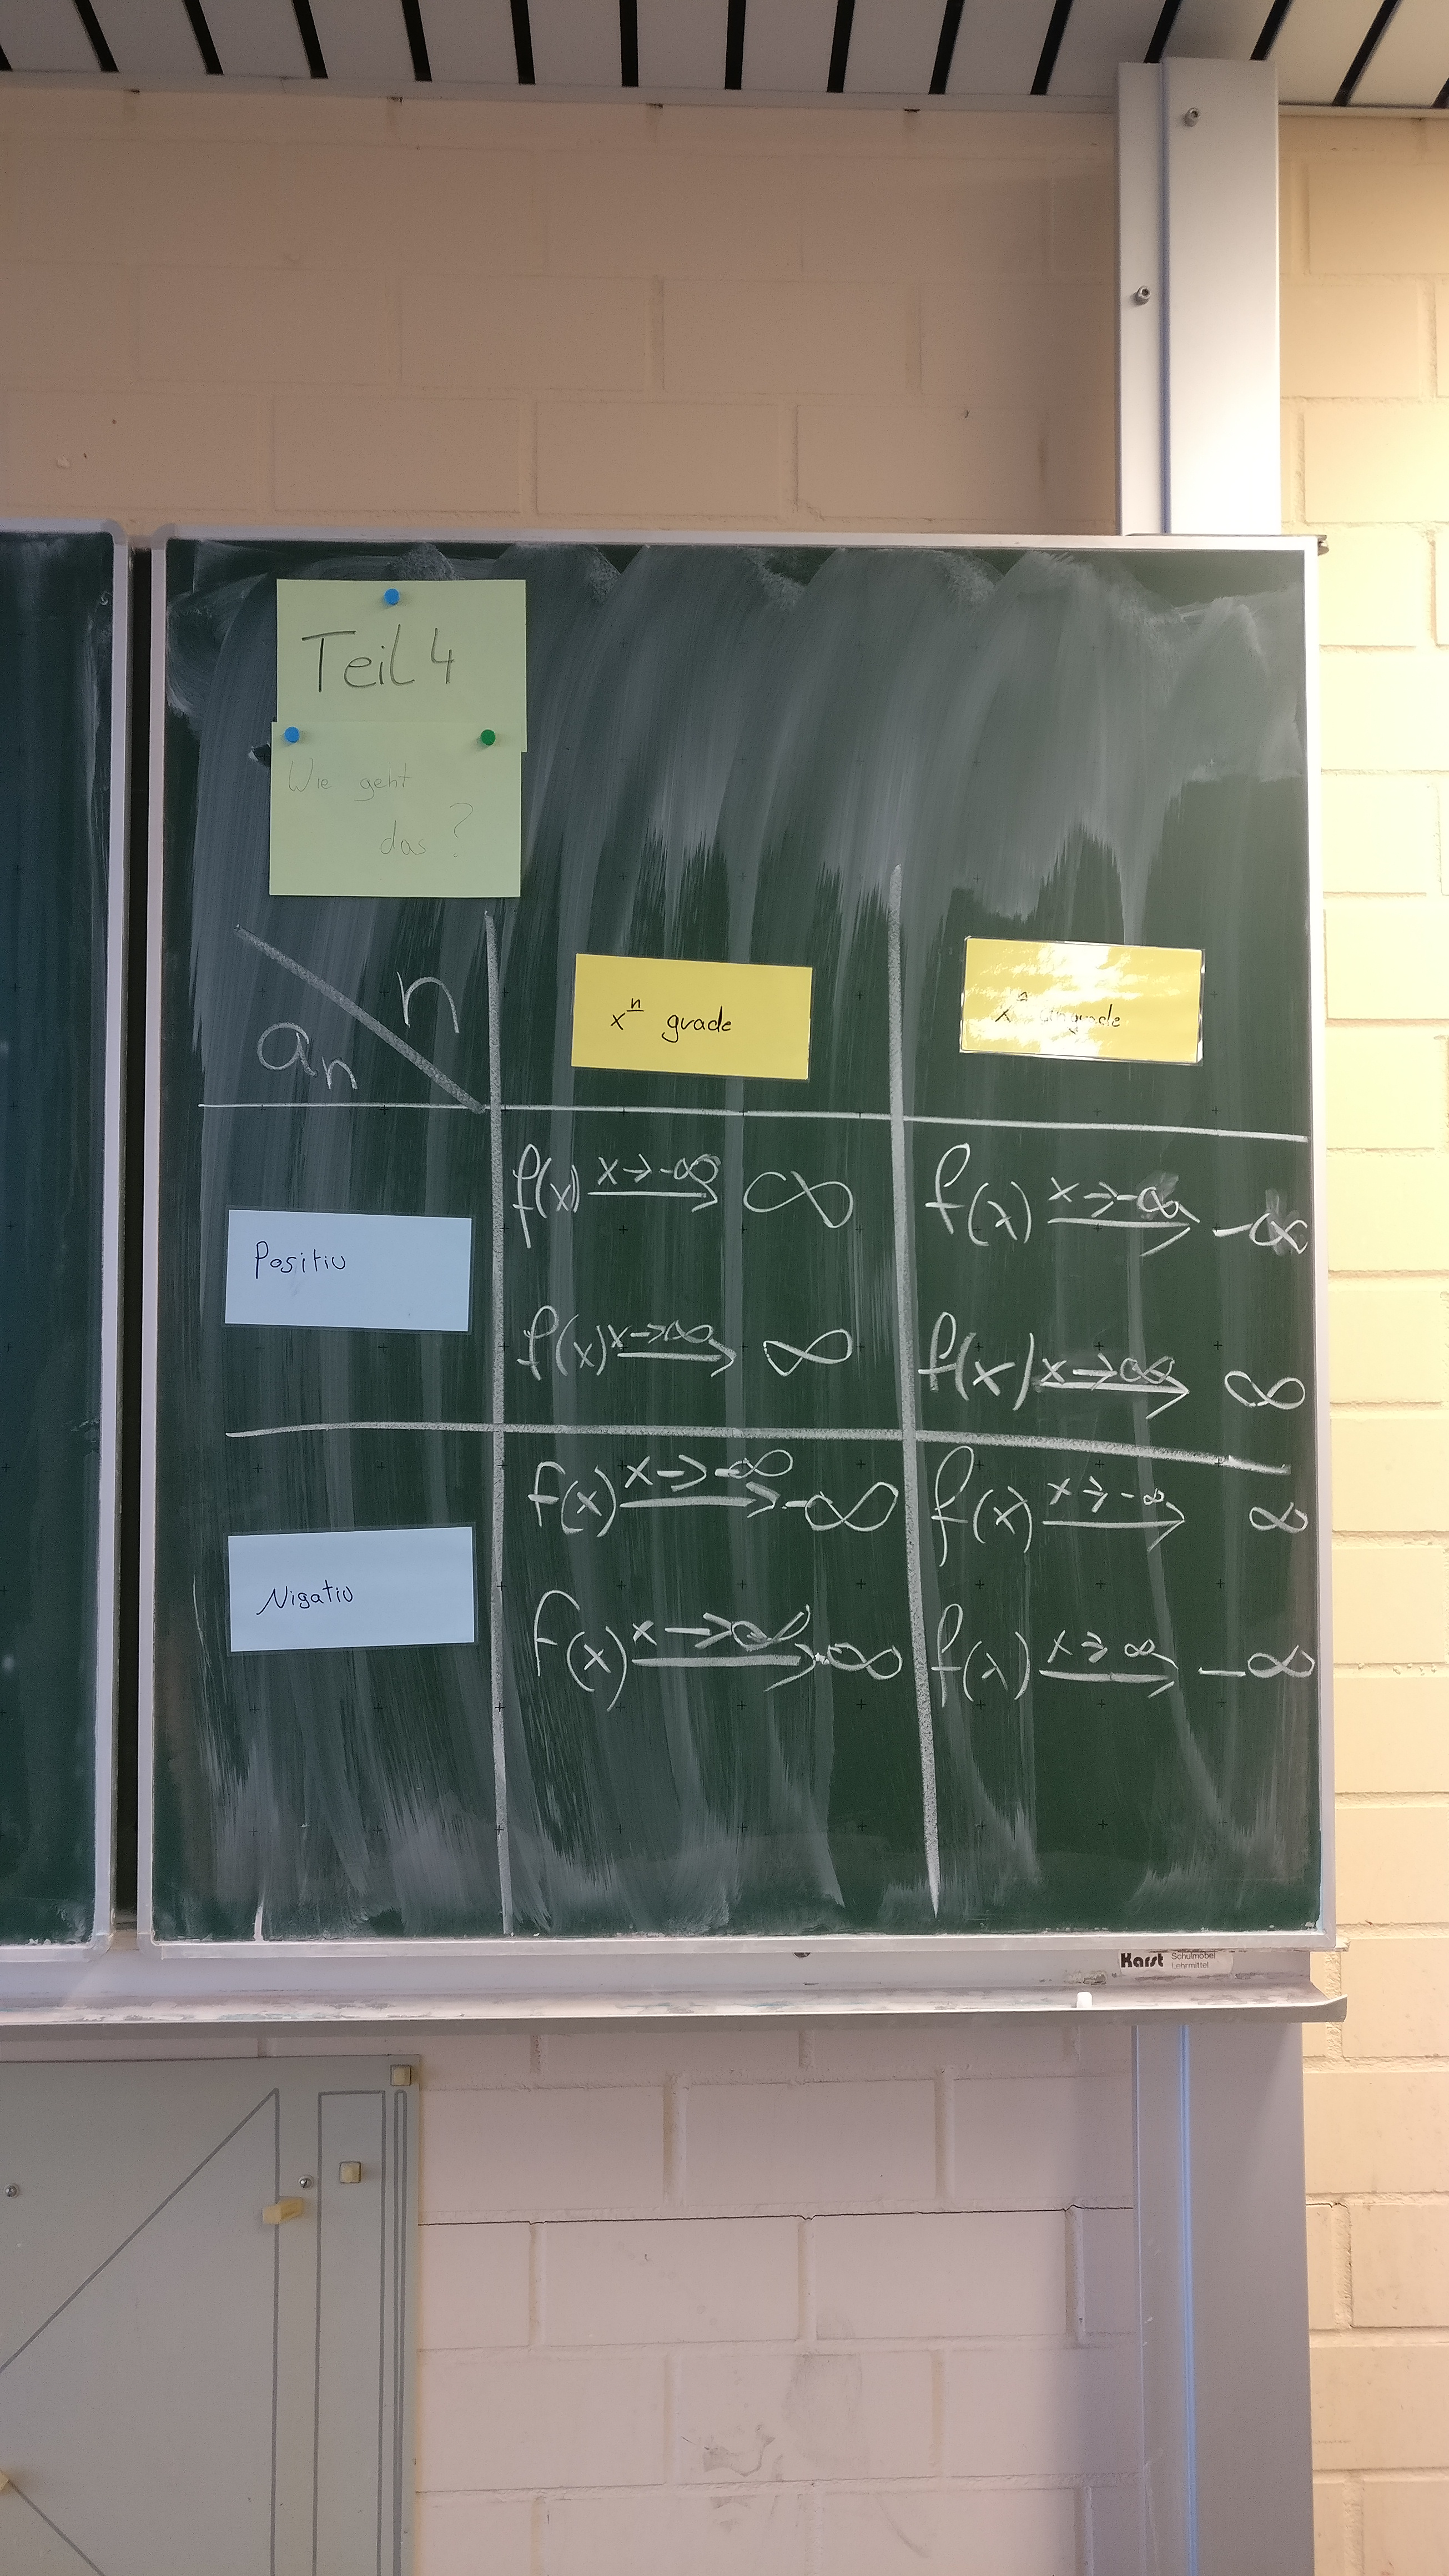
\includegraphics[width=0.34\textwidth]{../Tabelle_Verhalten.jpg}
		\end{center}
		In der Besprechung bzw. Plenumszeit war ich ausschließlich als Protokollant tätig. Die gesamte Besprechung wurde von den einzelnen Schülern moderiert und geleitet.\\
		\par\noindent
		\begin{minipage}{0.49\textwidth}
			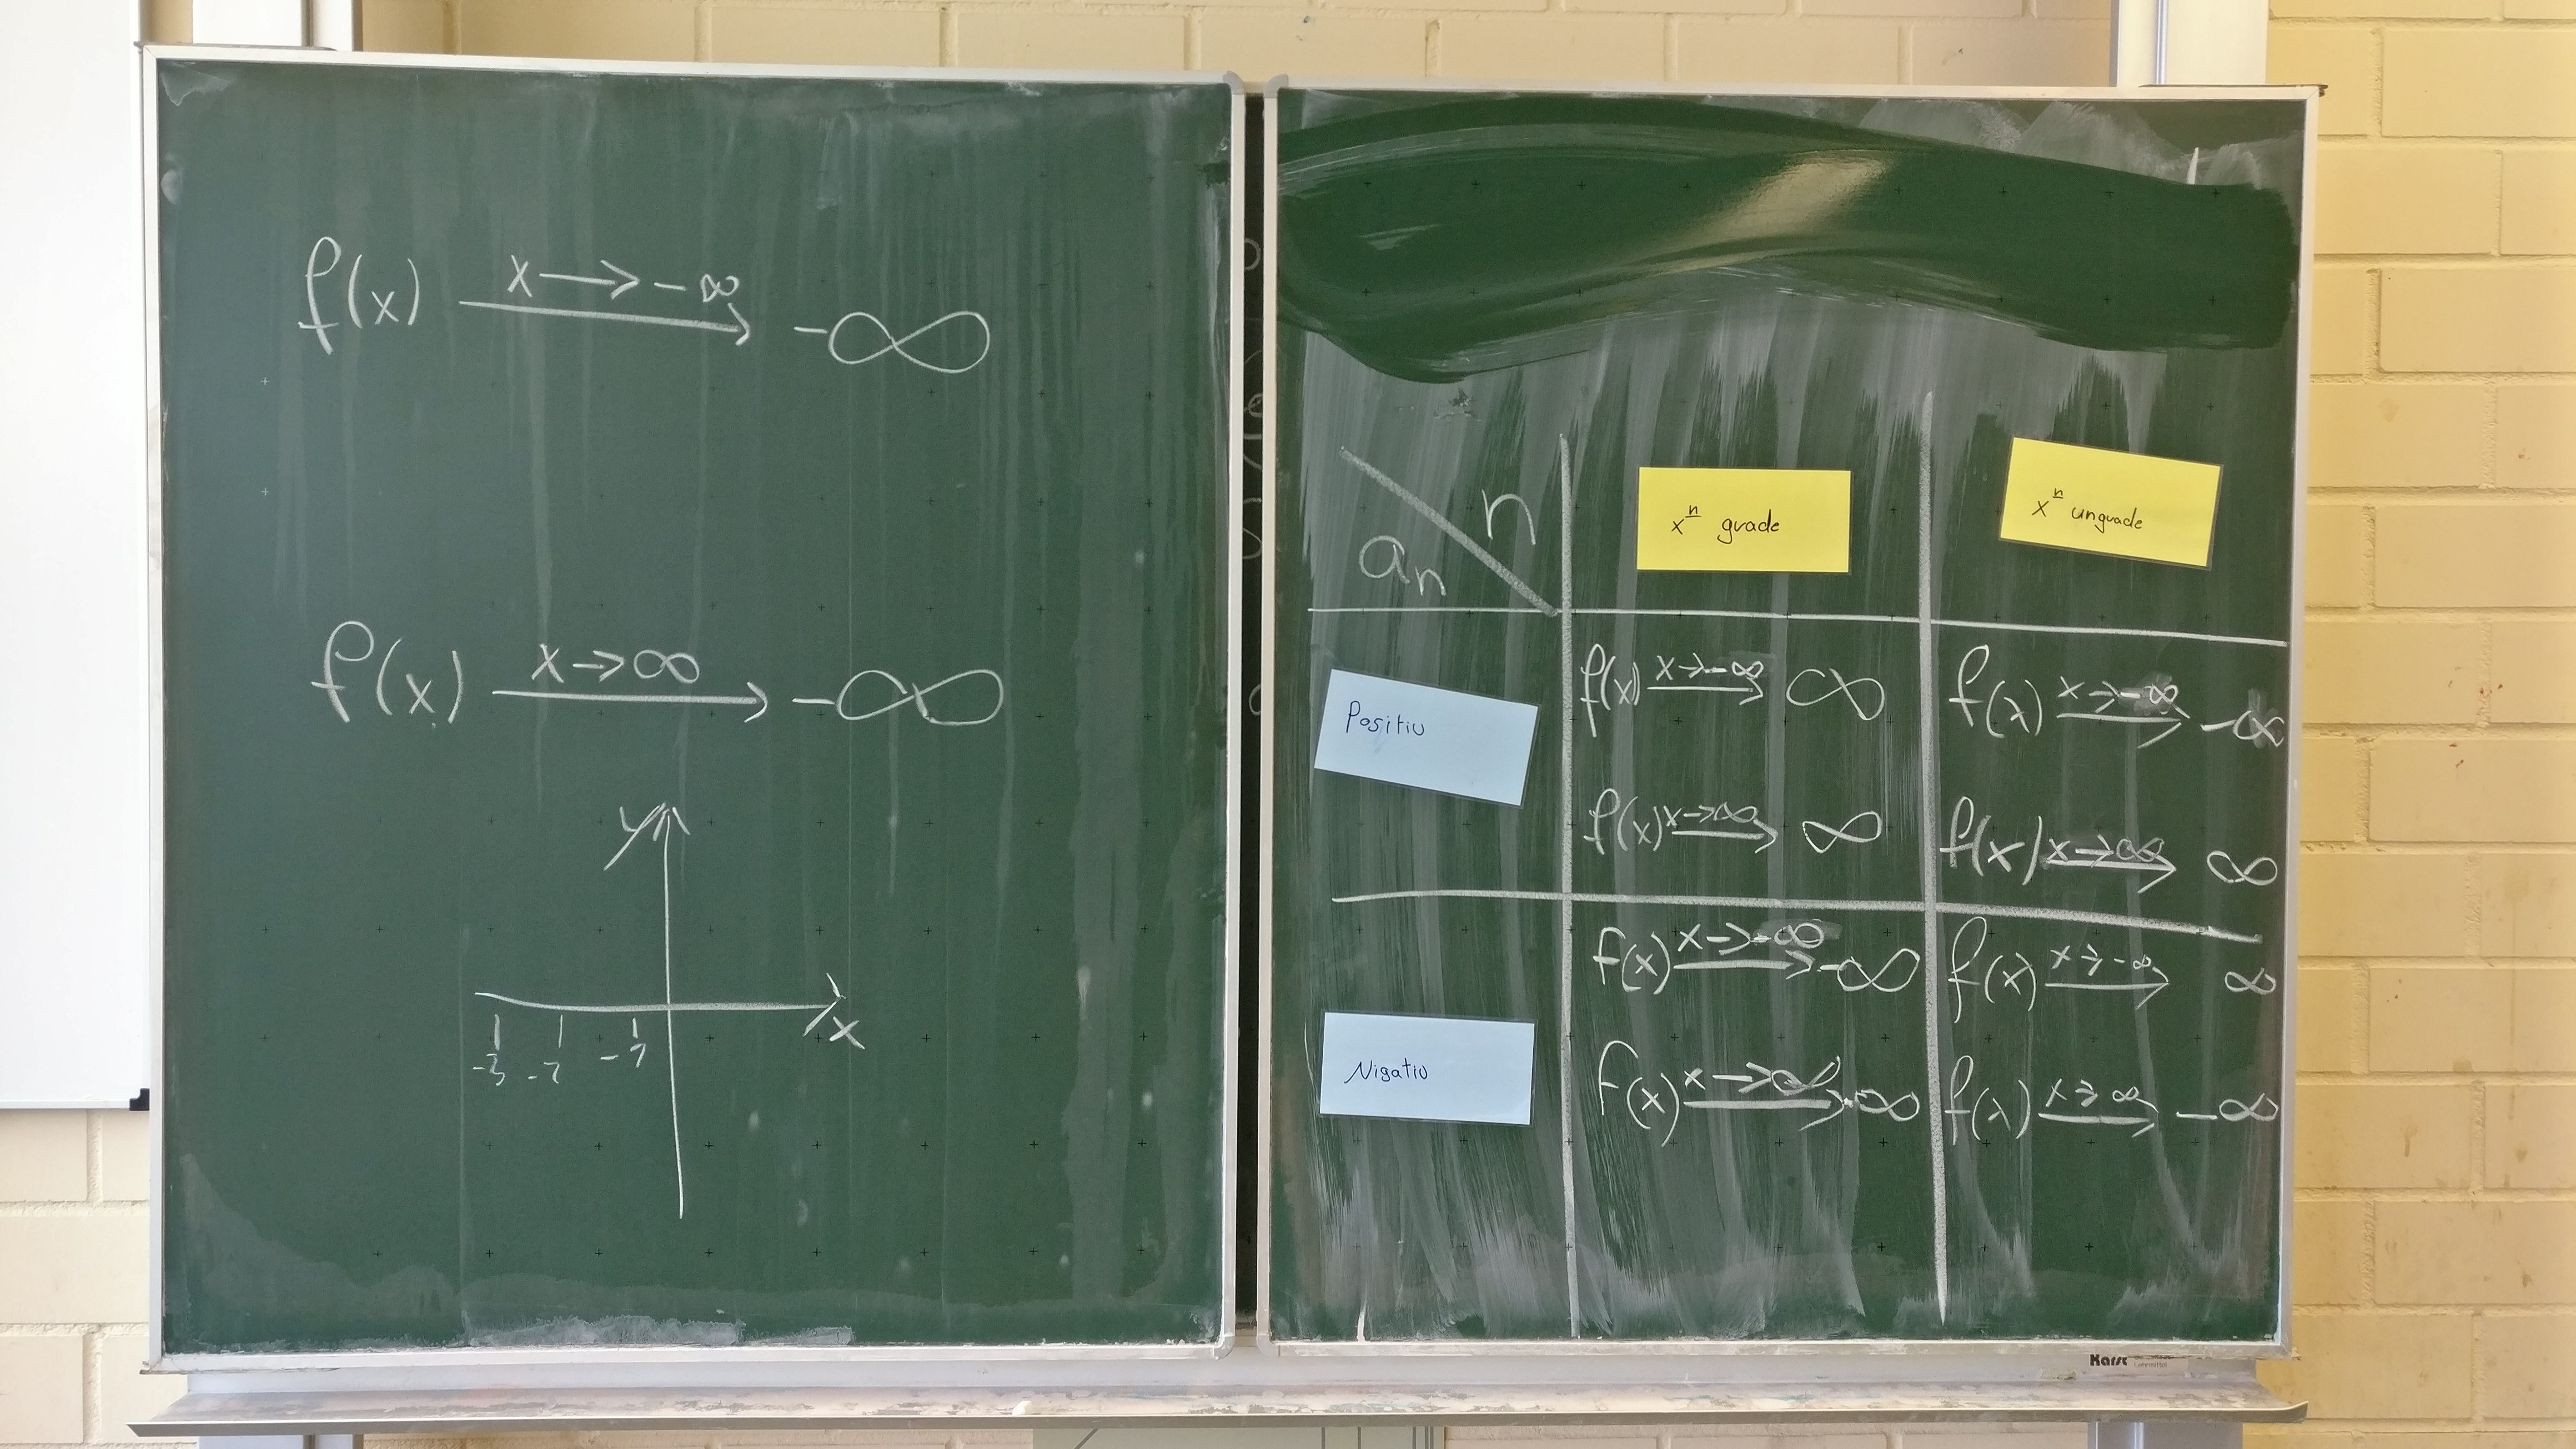
\includegraphics[width=\textwidth,align=t]{../Tabelle_VerhaltenMBsp.jpg}
		\end{minipage}
		\hfill
		\begin{minipage}{0.49\textwidth}
			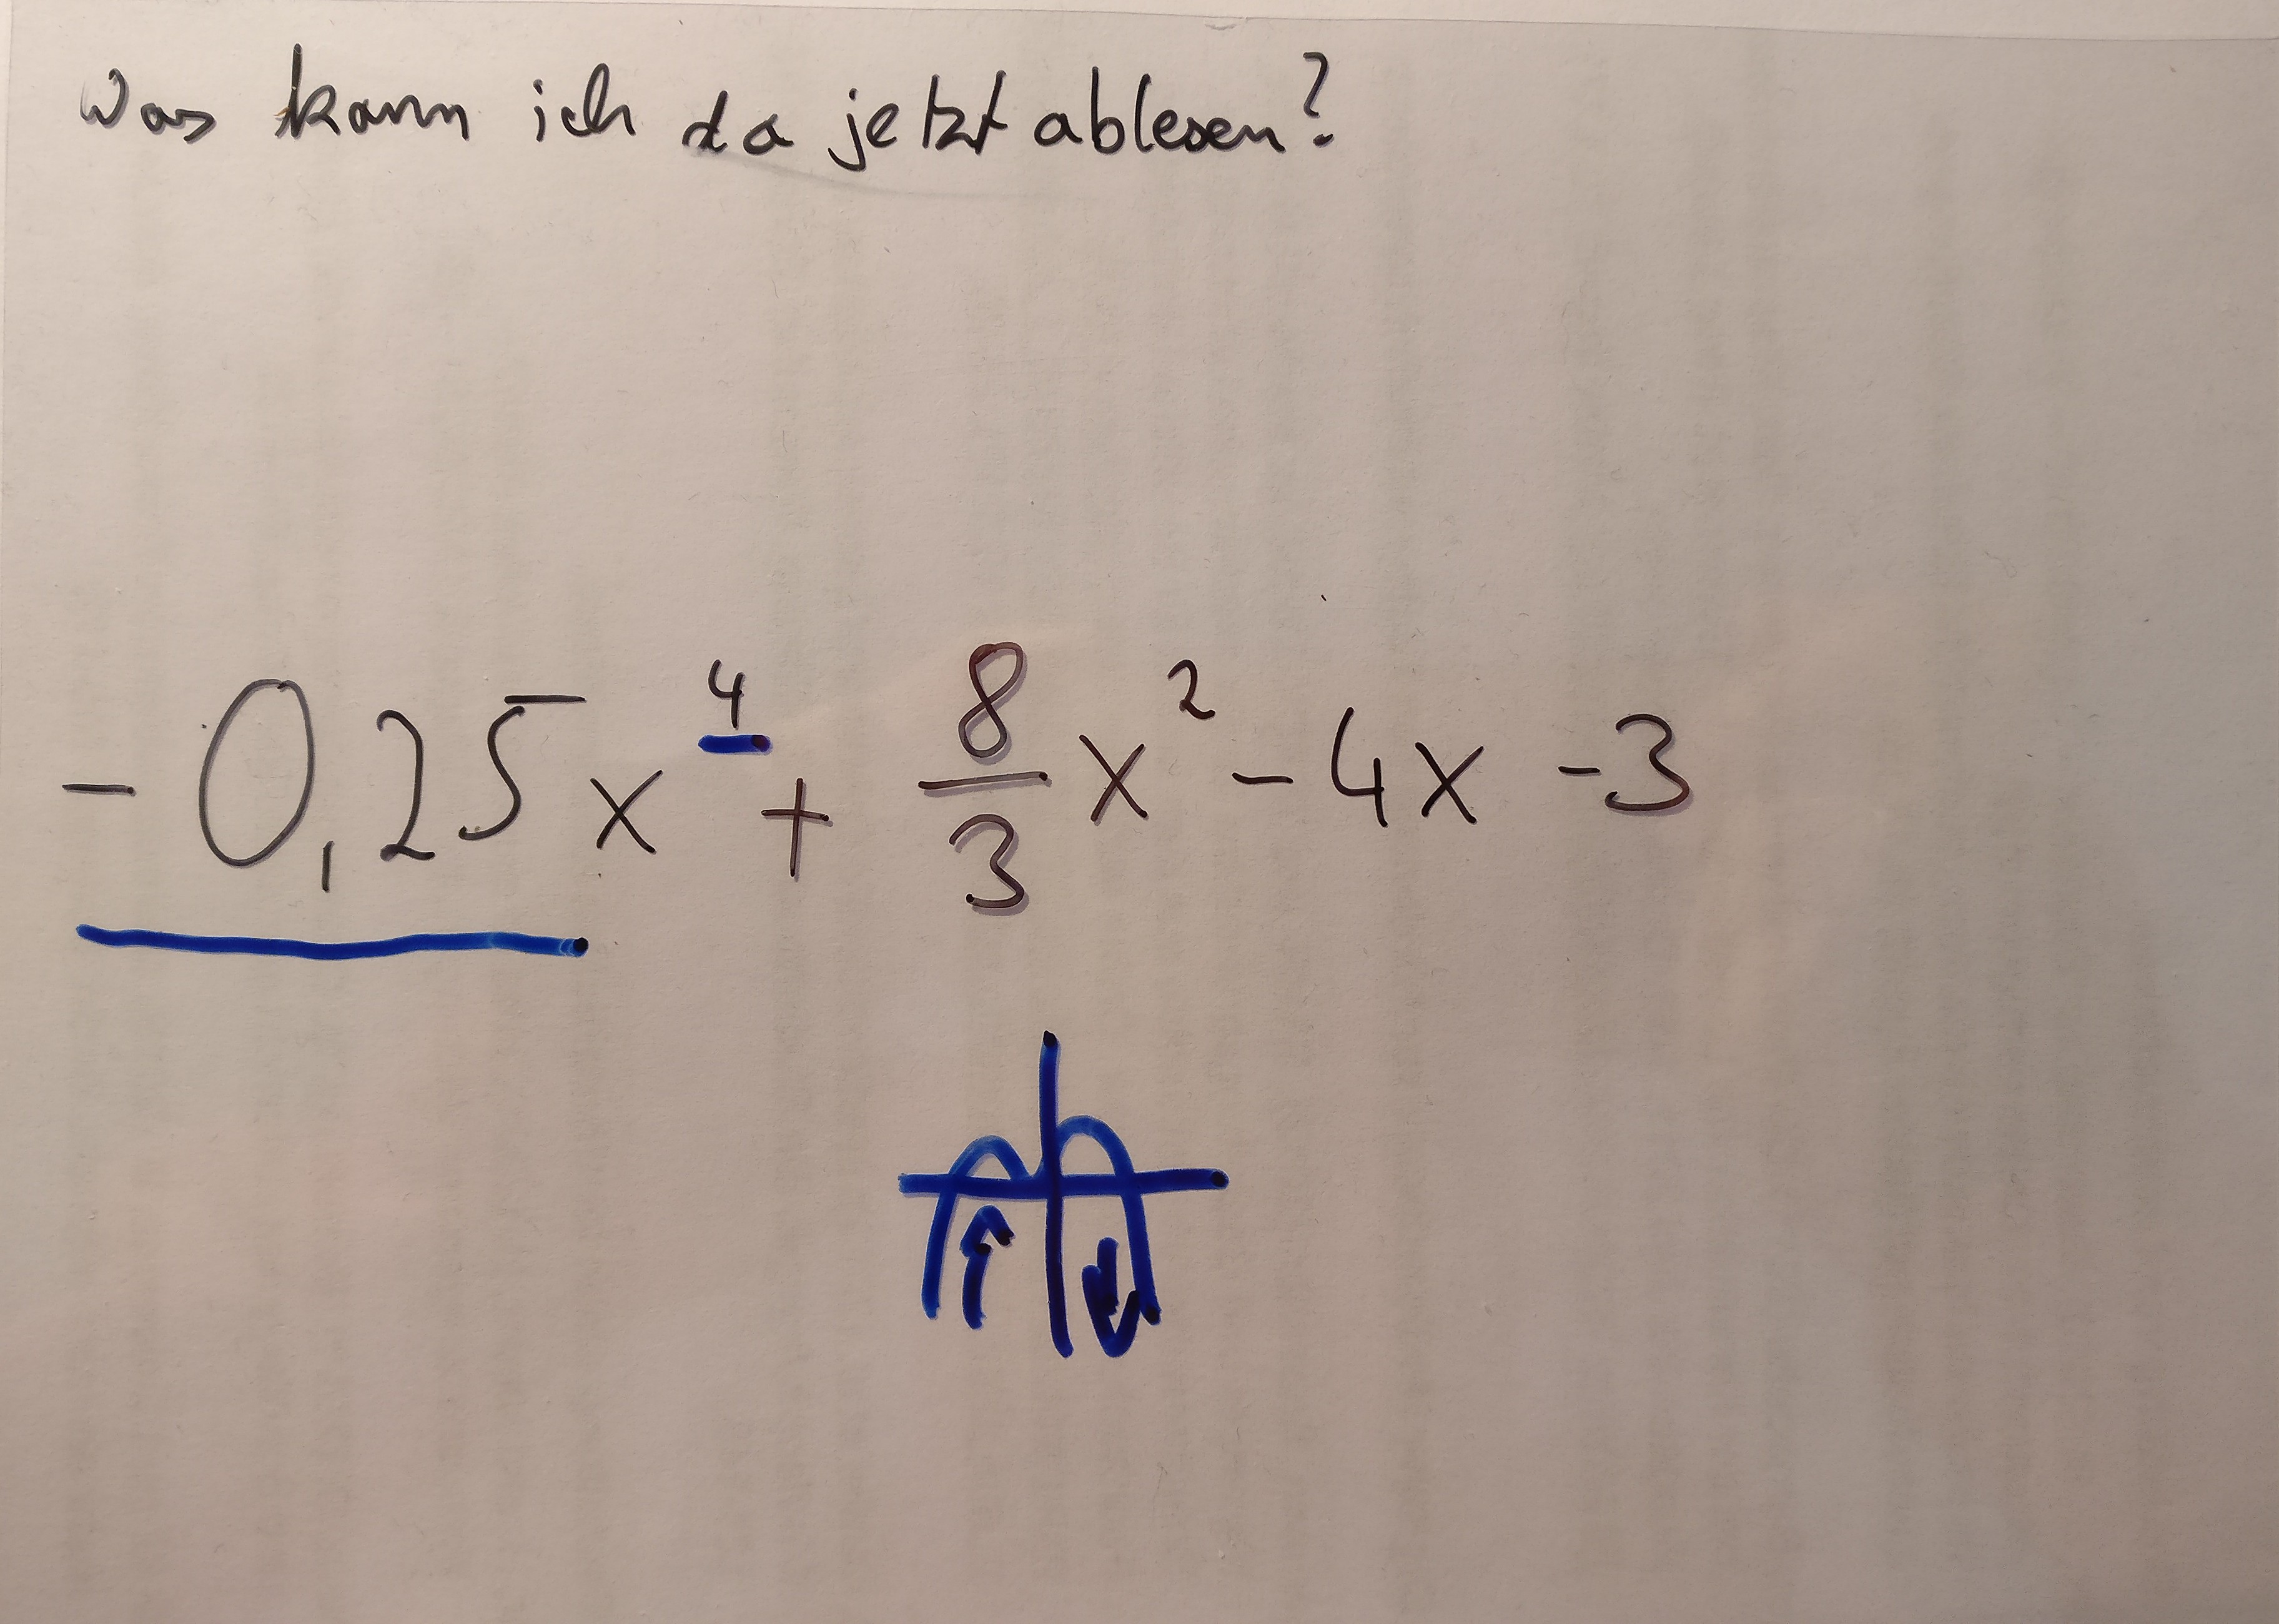
\includegraphics[width=\textwidth,align=t]{../VerhaltenAblesen.jpg}
		\end{minipage}\\
		\par
		\setlength{\leftskip}{1cm}
		\noindent
		\textit{\textbf{$\lbrack$Update: 19.12.2018$\rbrack$} Über die vergangene zwei Wochen habe ich diese Methode der Besprechung und des Austauschs genutzt.\footnote{Alle Ergebnisse der vergangenen zwei Wochen finden sich im Anhang.}\\
		Dabei gingen die Austauschphasen häufig eher schleppend von statten. Dies lässt sich leider dadurch erklären, dass eine Großzahl der Schüler die Hausaufgaben nicht oder nur sehr sporadisch bearbeitet haben.\\
		Daher waren die Schüler in der Austauschphase eher damit beschäftigt in Kooperation die Aufgaben des Wochenplans zu bearbeiten.\\
		Dieses Vorgehen tat aber der Besprechungsphase keinen Abbruch, da sich bei den Schülern während der gemeinsamen Bearbeitung dennoch Unklarheiten aufkamen. In der Besprechungsphase hingegen blühten die Schüler regelrecht auf. \textit{Dies mache ich besonders an der regen Beteiligung, auch durch schwächere Schüler fest.} Dabei konnte teilweise auch ein sonst eher leistungsschwächerer Schüler der Klasse eine Unklarheit aufklären.}
		\par
		\setlength{\leftskip}{0cm}
		\noindent
		
		\section*{\color{blue}{\ul{Können Schüler total selbstgesteuert Lernen?}}}
		\tiny{Geschrieben am: 01. Dezember 2018}\small\\
		\par\noindent
		Besonders im Rahmen der Planung meiner Unterrichtsreihe für meine Präsentationsprüfung habe ich mich des öfteren gefragt, inwieweit Schüler überhaupt dazu in Lage sind, sich selbst und ihren Lernprozess zu organisieren.\\
		Daher habe ich mich für den Dezember dazu entschieden den Unterricht in zwei meiner so vorzubereiten, dass der Wissenserwerb ausschließlich durch Eigenrecherche und Selbstorganisation (Verwendung von zur Verfügung gestellten Skripten, Informationsmaterialien) stattfindet.\\
		\par\noindent
		\color{ma}
		$\lbrack$\textbf{Mathematik}$\rbrack$ Die erste Klasse ist die HBF\footnote{HBF IT 18A}. Bisher habe ich den Schülern zu Lernabschnittsbeginn ein Skript zur Verfügung gestellt, in welchem sie die behandelten fachlichen Inhalte nachschlagen können. Diese Skripts wurden durch mich aber während des Unterricht nicht explizit verwendet. Den Schülern war aber freigestellt, diese bei der Bearbeitung zu verwenden.\\
		Im Zuge der Unterrichtsreihe zur Präsentationsprüfung habe ich den bisher genutzten Wochenplan so angepasst, dass die Schüler die Aufgaben in Gänze alleine bearbeiten können.\\
		\par\noindent
		\color{iv}
		$\mathbf{\lbrack}$\textbf{Informatik}$\mathbf{\rbrack}$ Im Informatikgrundkurs der Jahrgangsstufe 12\footnote{BGY 17 - iv2} habe ich ebenfalls jeden Lernabschnitt mit einem bzw. mehreren Skripts unterstützt. Dabei lag hier der Schwerpunkt aber eher auf einer gemeinsamen Erarbeitung\footnote{Dabei heißt gemeinsam, dass die Schüler Arbeitsgruppen formen, in denen Sie gemeinsam an der Aufgabenstellung arbeiten.} der Problemlösung liegt.\\
		\normalcolor
		\section*{\color{blue}{\ul{Präventive Maßnahme bei Störungen}}}
		\tiny{Geschrieben am: 22. November 2018}\small\\
		\par\noindent
		\begin{wrapfigure}{L}{0.25\textwidth}
			\centering
			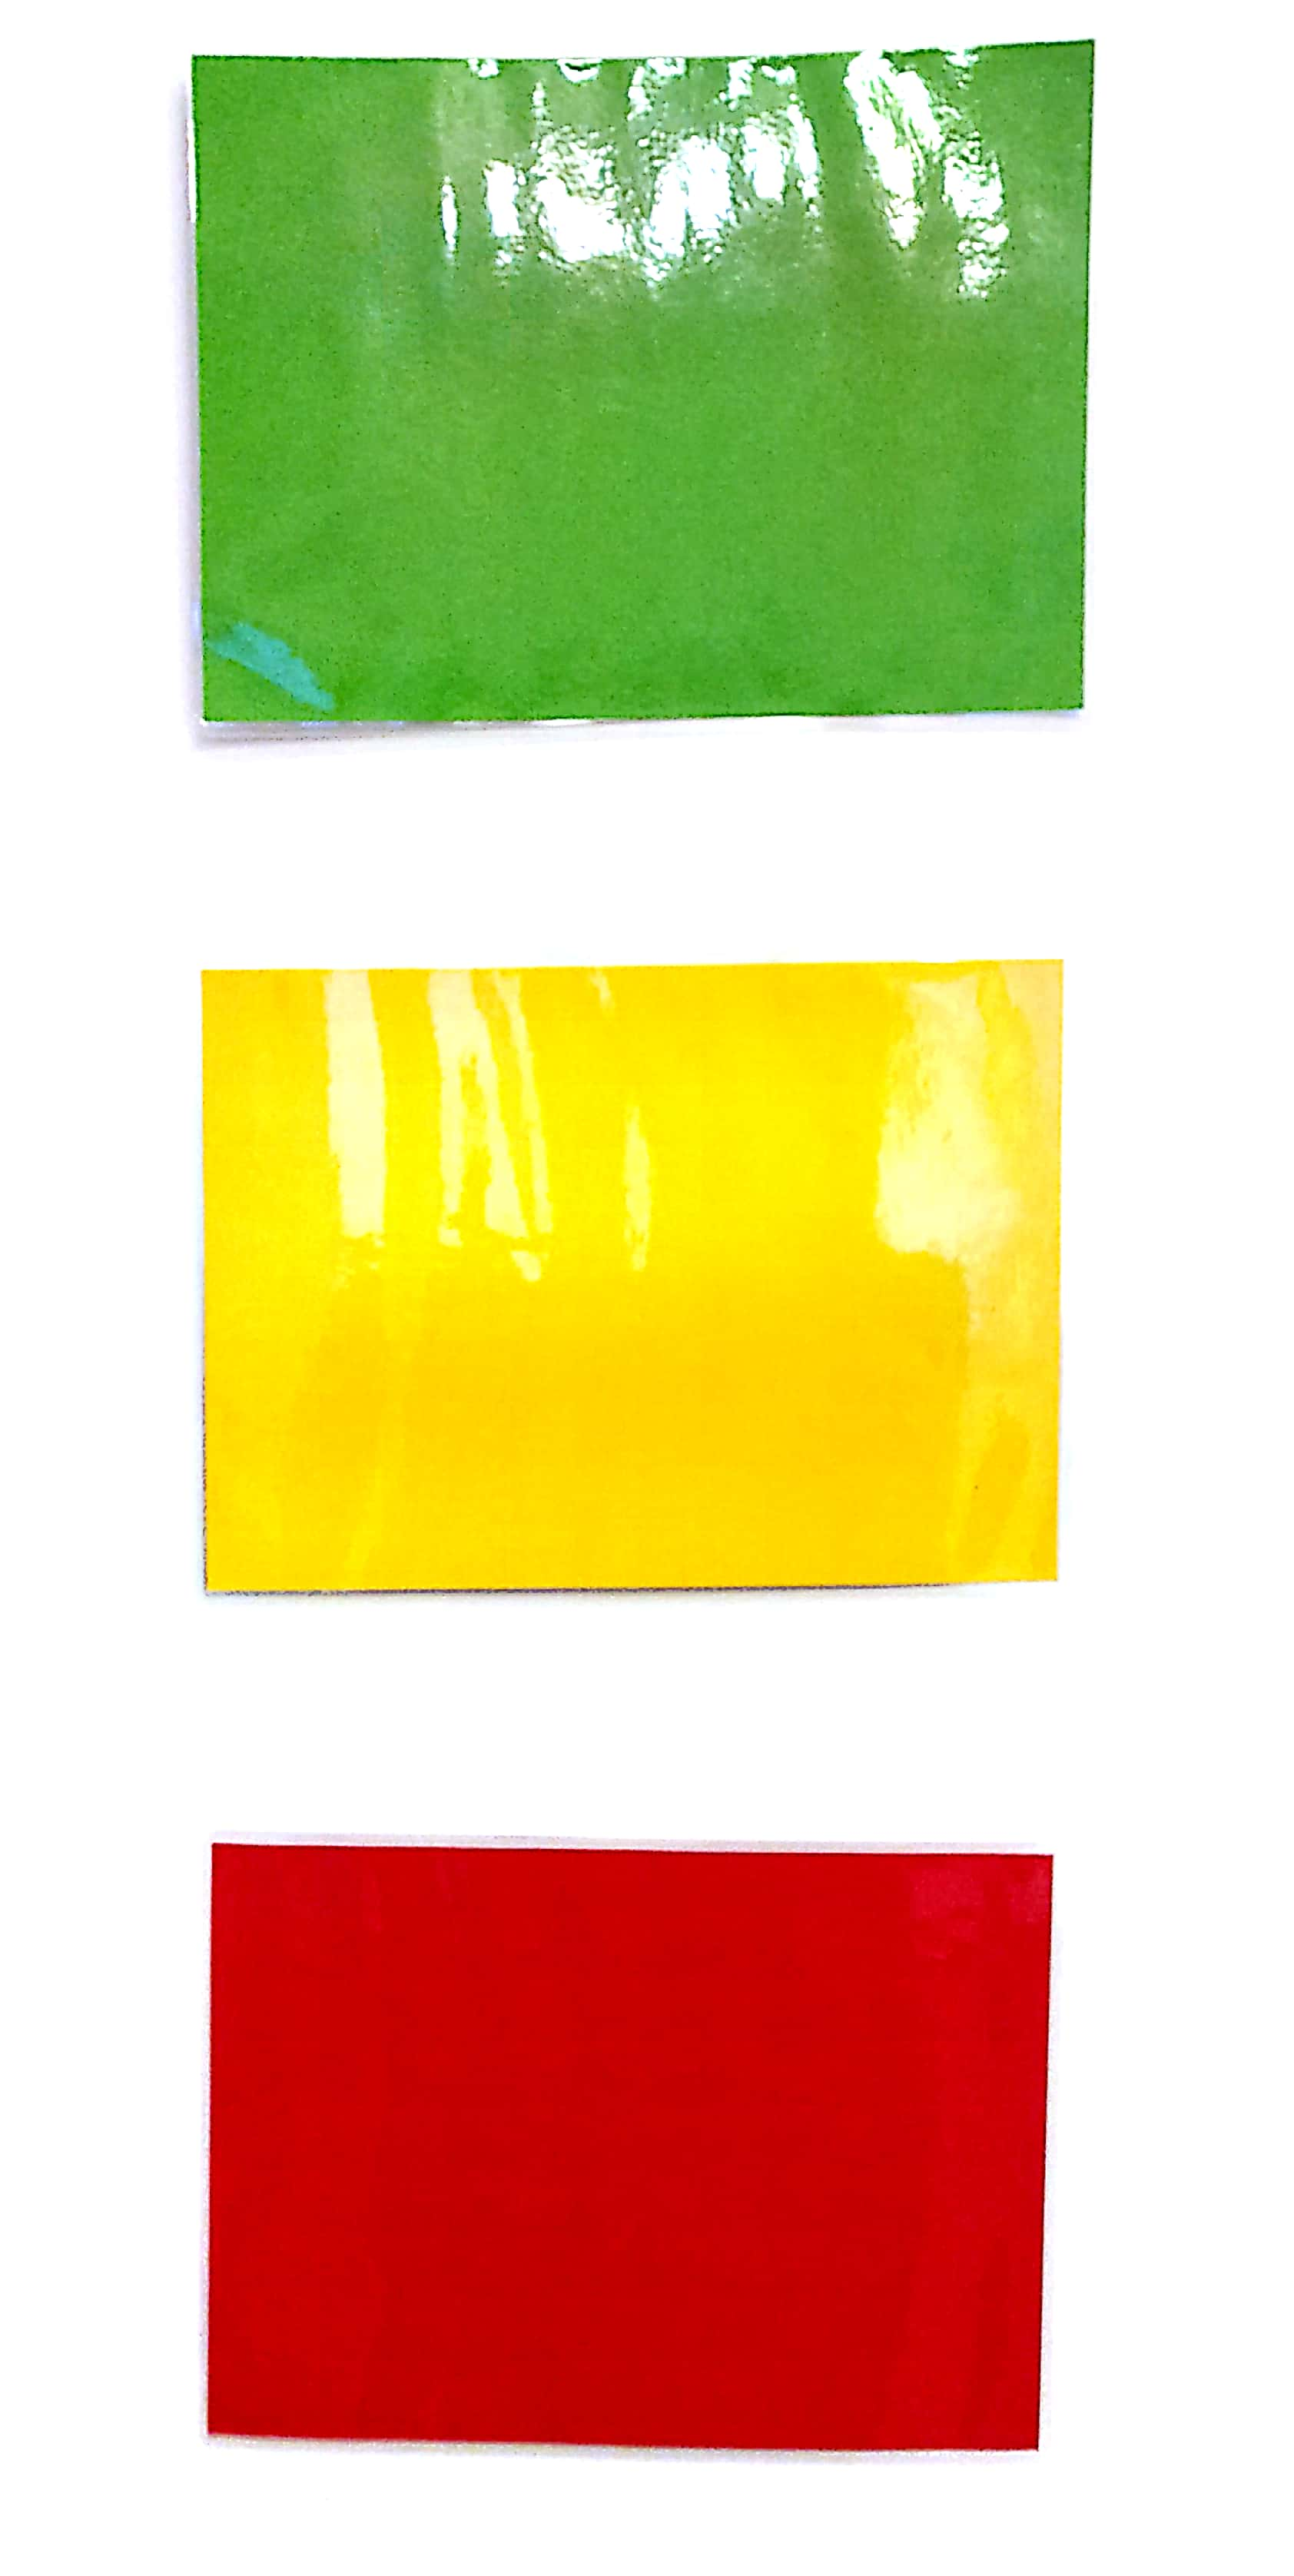
\includegraphics[width=0.15\textwidth]{LSA.jpg}
		\end{wrapfigure} Da die Schüler meiner HBF\footnotemark[1] häufig in Partnerarbeit, von Zeit zu Zeit aber auch in Einzelarbeit, an der Problemlösung arbeiten, habe ich zeitnah nach Schuljahresbeginn eine Lautstärkeampel eingeführt. Diese soll dazu beitragen eine Arbeitsatmosphäre zu schaffen, in der jeder unter akzeptablen Rahmenbedingungen arbeiten kann.\\
		\par\noindent
		Diese Ampel wird über farbige A5 Karten an der Tafel repräsentiert. Dabei starten die Schüler mit der \textbf{grünen} Karte in eine Arbeitsphase. Erreicht die Lautstärke einen Pegel, bei welchem ein effektives Arbeiten nicht möglich ist, oder aber die Schüler beschäftigen sich mit außermathematischen Dingen, folgt zunächst eine gezielte verbale Ermahnung der Schüler. Kommt es unter den zuvor ermahnten Schülern erneut zu Störungen, tausche ich die \textit{grüne} durch eine \textbf{gelbe} Karte aus.\\
		Diesen Wechsel kommuniziere ich auch den Schülern, so dass ihnen bewusst ist, dass sie sich unangemessen verhalten haben. Ebenso teile ich ihnen mit, dass sie für die verbleibende Zeit unter besonderer Beobachtung stehen.\\
		Die nachfolgenden Ermahnung dieser Schüler erfolgen nur noch auf non-verbaler Ebene (beispielsweise durch \grq{}penetranten\grq{} Blickkontakt oder langsames Annähern an die Schülergruppe meinerseits). Zeigen diese Ermahnungen keine Reaktion, so erfolgt der Wechsel von \textit{gelb} auf \textbf{rot} ohne weitere Warnung.
		\par
		\setlength{\leftskip}{1cm}
		\noindent
		\textbf{$\lbrack$Update: 29.11.2018$\rbrack$} Wie im Jahresgespräch angemerkt, habe ich im Unterricht am vergangenen Dienstag eine Alternative zu der \grqq{}Strafe\grqq{}\footnote{Bisher war dies ein Test in der darauffolgenden Stunde.} bei erreichen der \textit{roten} Karte eingeführt.
		\textit{In der Klasse habe ich die Schüler nach den Herbstferien über den Unterrichtsverlauf bis zu den Weihnachtsferien informiert. Hierzu zählte auch, dass ich diverse kleinere Tests angekündigt habe. Zum einen sollten diese Tests mir dabei helfen, den Leistungsstand der einzelnen Schüler besser beurteilen zu können und gegebenenfalls Anpassungen im weiteren Unterrichtsverlauf vorzunehmen. Zudem sollten die Schüler dazu angeleitet werden, sich in Vorbereitung auf den anstehenden Test noch einmal mit den Unterrichtsmaterialien auseinanderzusetzen. Auf diese Weise haben die Schüler bei der Vorbereitung für die Klassenarbeit nicht soviel nachzubereiten, da sie sich im Verlauf des Schuljahres immer wieder mit den Materialien auseinandersetzen.}
		\par
		\setlength{\leftskip}{0cm}
		\noindent
		Für die vergangene Stunde habe ich den Schülern vor Beginn der Arbeitsphase mitgeteilt, sollten sie die Arbeitsphase mit der \textit{günen} Karte beenden, so werden wir den angekündigten Test zwar schreiben, es wird aber keine Benotung stattfinden.\\
		Dieses Vorgehen wurde von den Schülern dankend angenommen und führte während der Arbeitsphase zu einer gegenseitigen Ermahnung der Schüler durch andere Schüler.
		
		\section*{\color{blue}{\ul{$\lbrack$Mathematik$\rbrack$ Kann ein cheat-sheet die Schüler bei der Klausur unterstützen?}}}
		\tiny{Geschrieben am: 10. November 2018}\small\\
		\par\noindent
		Am gestrigen Tag stand im 13er Grundkurs des BGY\footnote{\textbf{B}erufliches \textbf{Gy}mnasium} die obligatorische Klausur an. Da der Unterricht immer Freitags in den Stunden 5., 6. und 7. stattfindet, habe ich unter der Woche keine zusätzliche Möglichkeit, Fragen der Schüler im Plenum zu besprechen.\\
		Üblicherweise beschäftigen sich die Schüler bis kurz vor der Klausur mit den Unterrichtsmaterialien, so dass das kürzlich angeschaute meist am Besten abrufbar ist. Daher habe ich mich dazu entschieden, die Klausur in der 6. und anschließenden 7. Stunde zu schreiben.\\
		\par\noindent		
		In der Vorstunde (also der 5. Stunde) haben ich den Schülern die Möglichkeit gegeben, dringende Fragen zu klären.\\
		Hierbei hat sich gezeigt, dass viele Schüler die fachlichen Inhalte abrufbar hatten, für diesen Prozess aber einige Zeit brauchen. Dadurch stellen die Schüler die Forderung, die Fragen und deren Antworten während der Klausur an der Tafel stehen zu lassen.\\
		\par\noindent
		Spontan habe ich mich dann dazu entschieden, den Schülern einen A6 \grq{}Spickzettel\grq{} zu erlauben. Die letzten 15 Minuten der 5. Stunde habe ich den Schülern zugestanden, um ihren \grq{}Spickzettel\grq{} mit für Sie relevanten Inhalten zu füllen. Dieser sollte mit der Klausur abgegeben werden.\\
		\par
		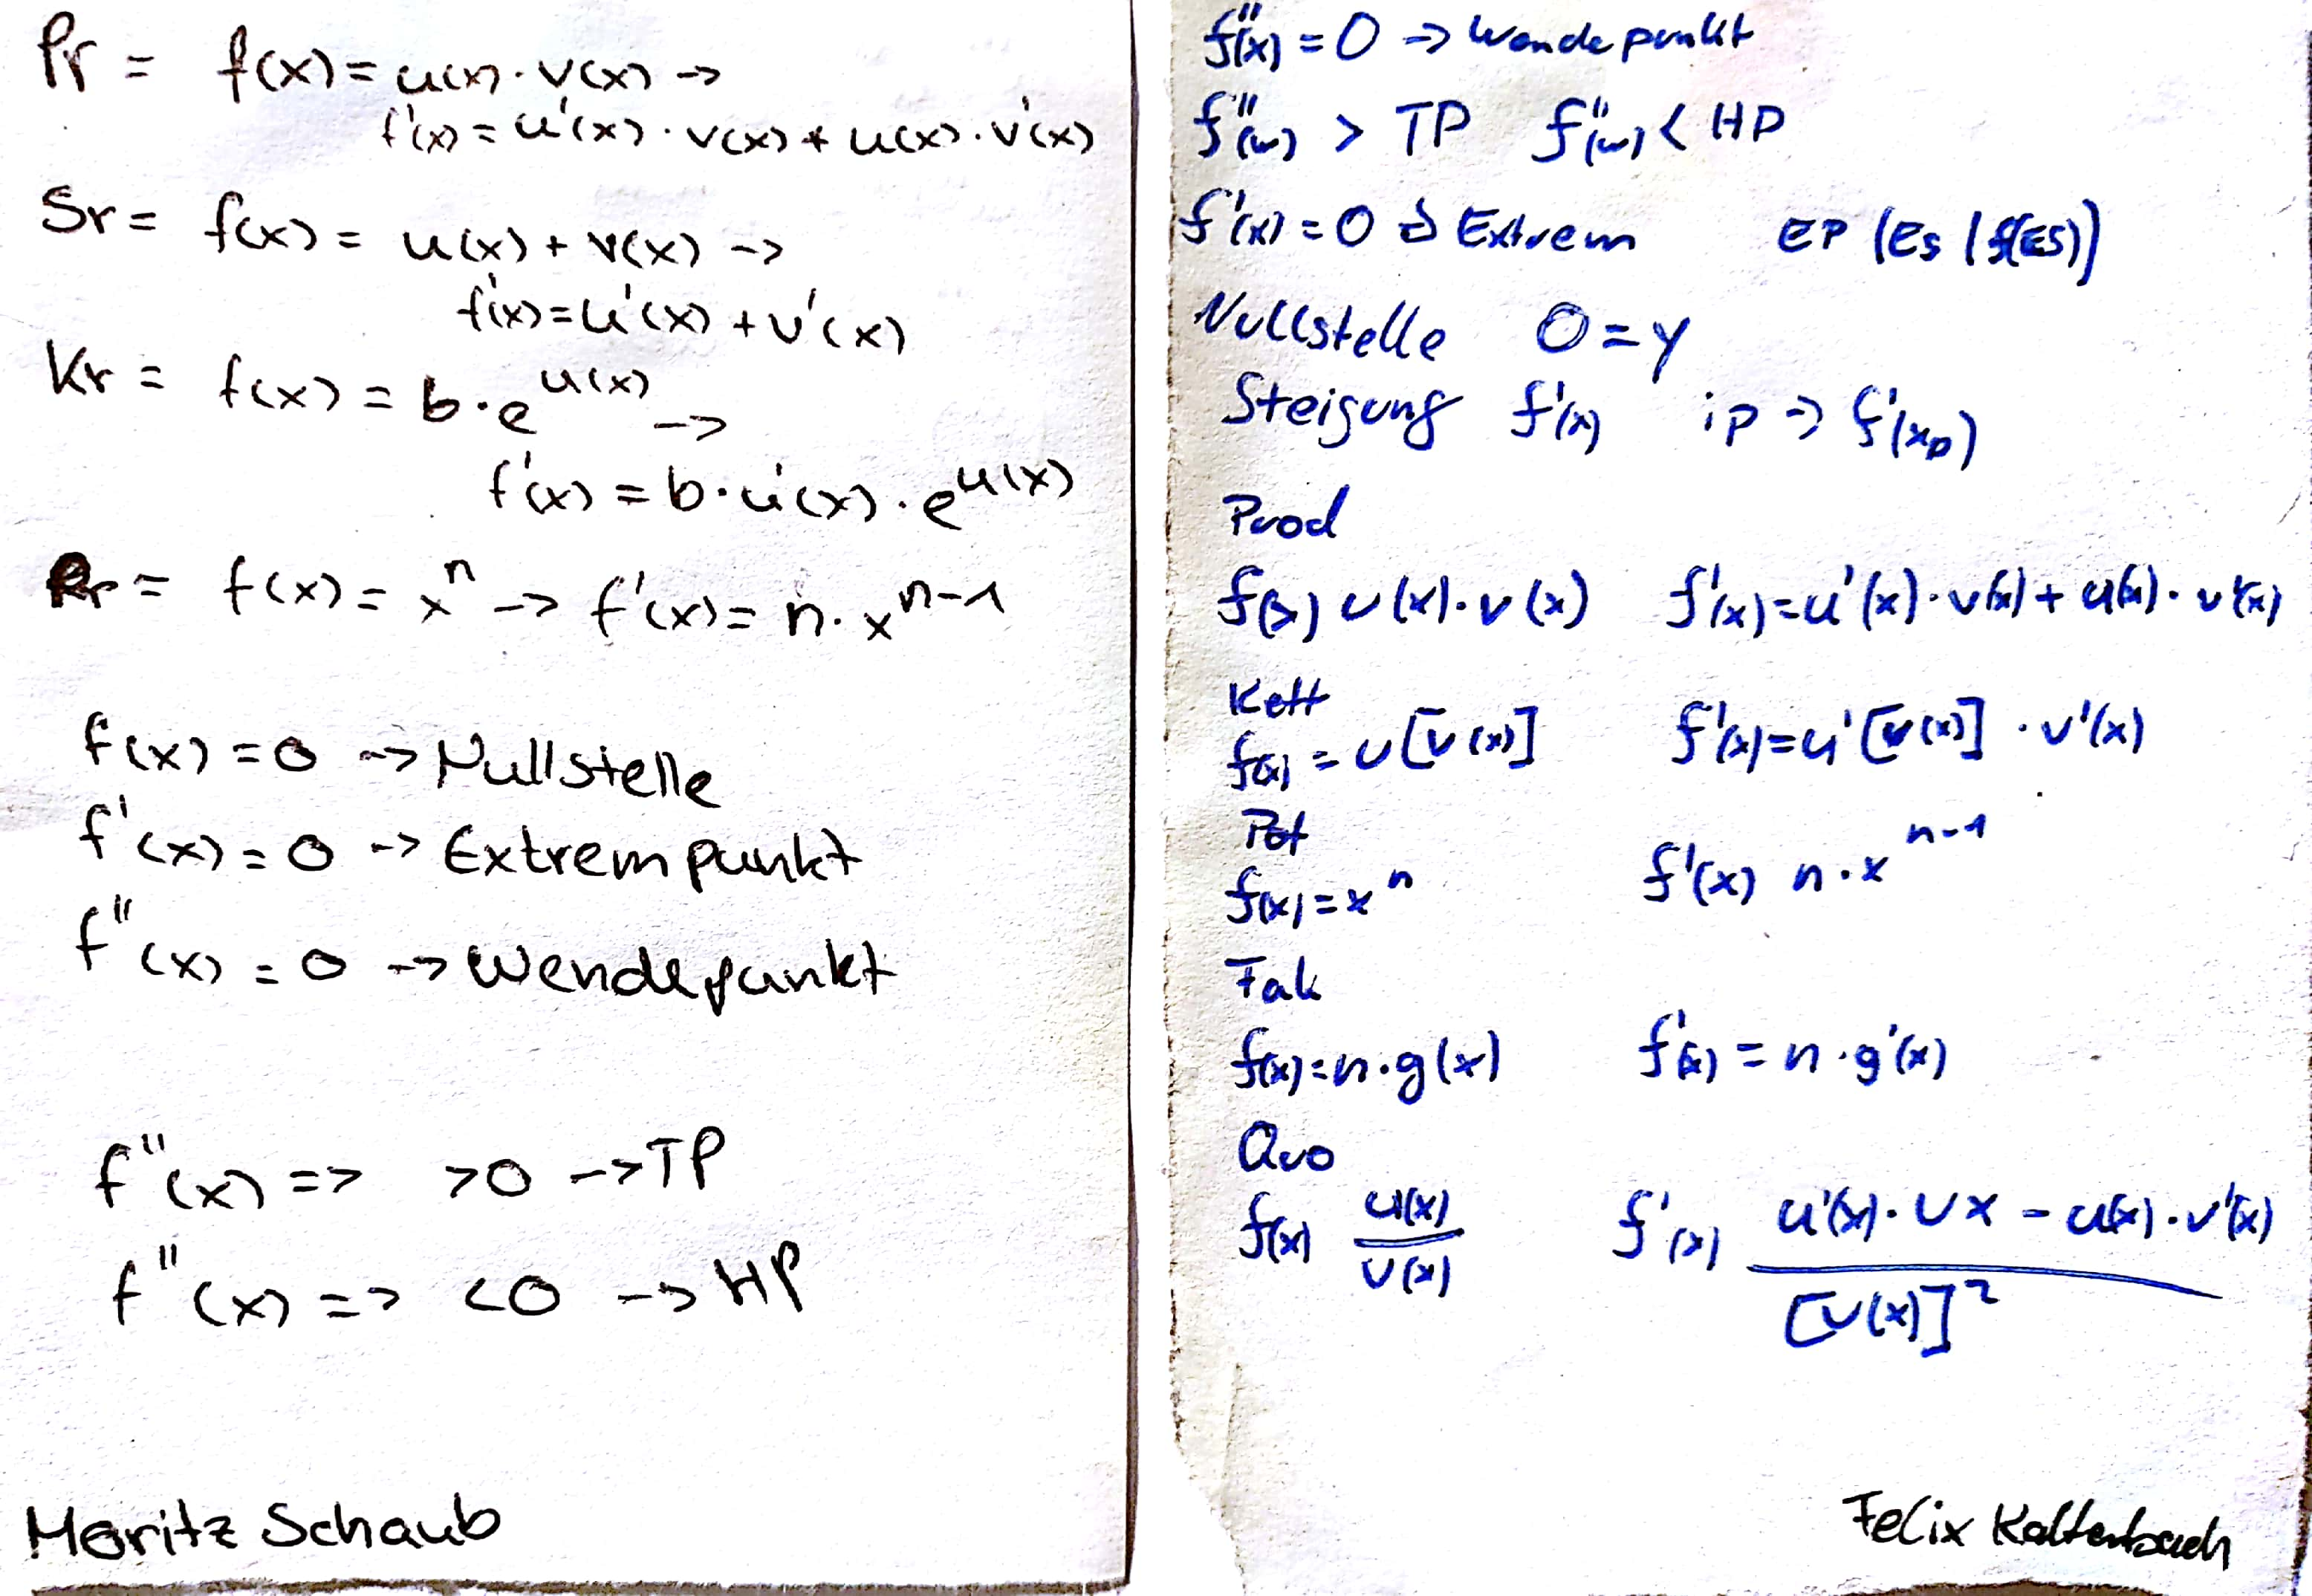
\includegraphics[width=\textwidth]{SpZ1.jpg}\\
		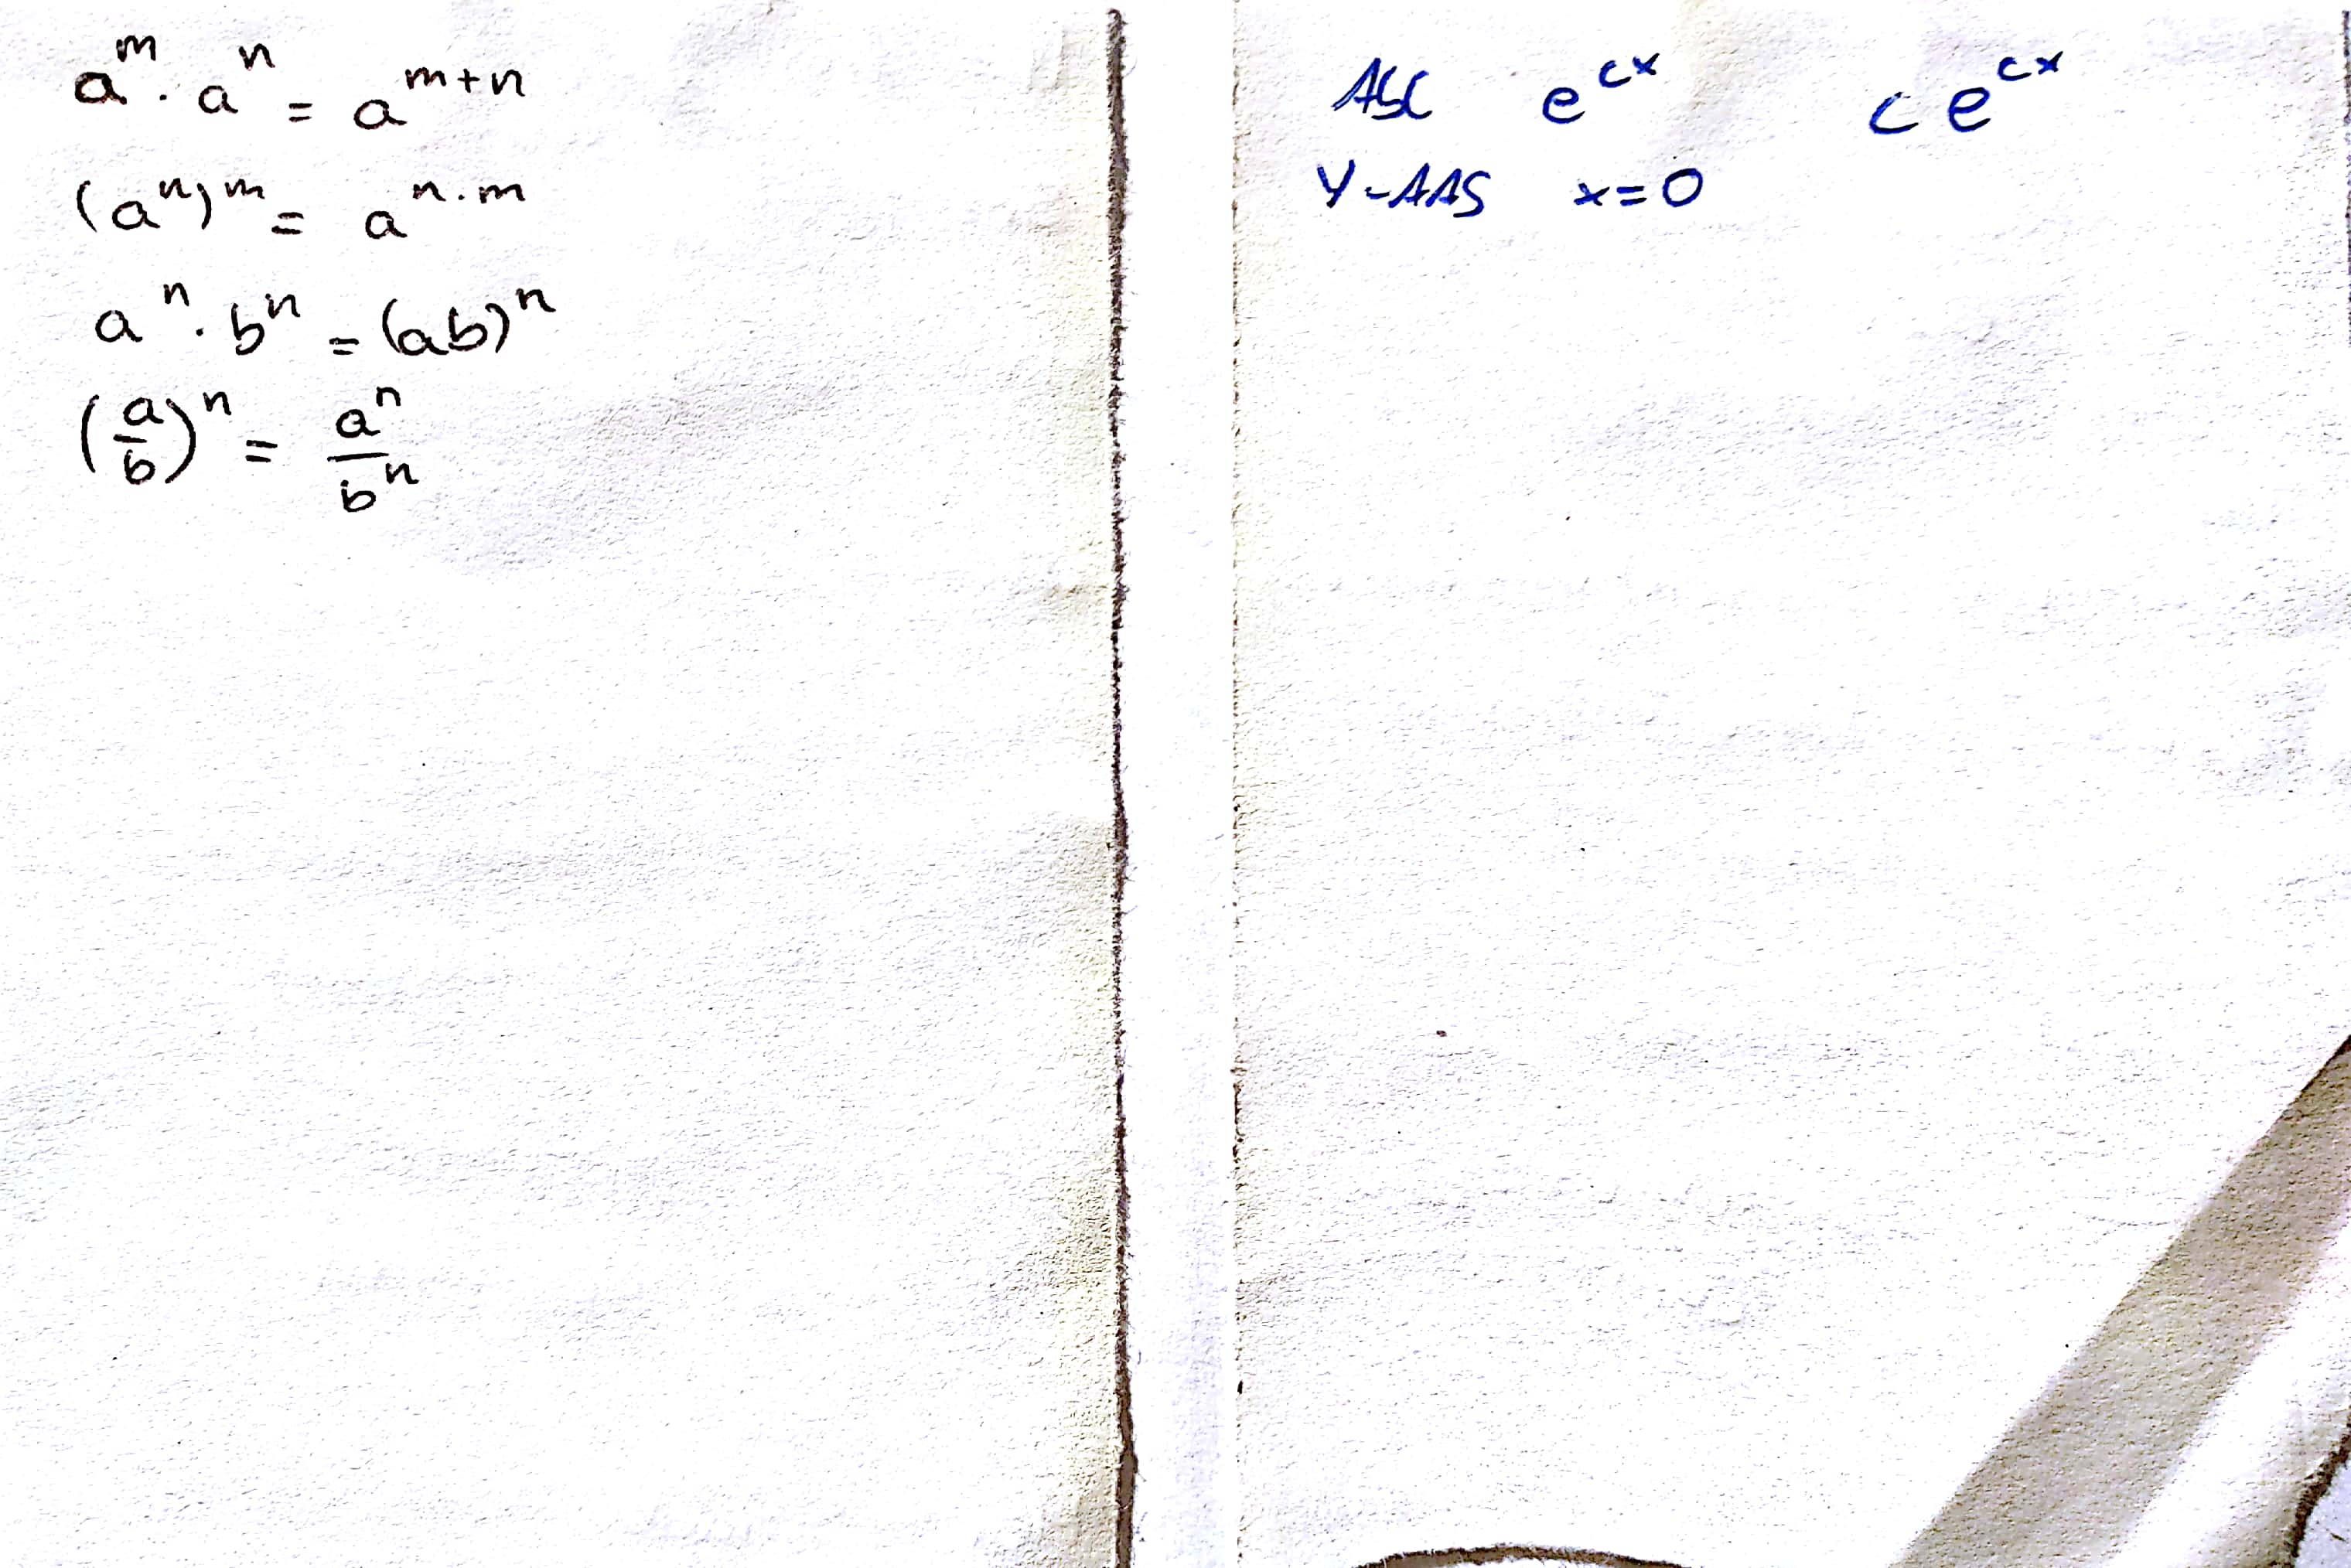
\includegraphics[width=\textwidth]{SpZ2.jpg}\\
		Dies sind nur zwei der insgesamt 20 \grq{}Spickzettel\grq{}. Die übrigen weisen aber ähnliche Hilfestellungen auf.\\
		\par\noindent
		Wir begannen pünktlich mit der Klausur. Eigentlich war ich davon ausgegangen, dass die Schüler verhältnismäßig gut mit den Aufgaben zurecht kommen würden. Während der Bearbeitungszeit hat sich gezeigt, dass ich die Fähigkeiten und Kompetenzen des Kurses leicht überschätzt habe.
		\par
		\setlength{\leftskip}{1cm}
		\noindent
		\textbf{$\lbrack$Update: 16.11.2018$\rbrack$} Bei der Korrektur hat sich aber gezeigt, dass ich den Kurs zum einen überschätzt habe und die Schüler trotz des erlaubten \grq{}Spickzettels\grq{} nicht in der Lage waren, die erarbeiteten Vorgehensweisen nicht auf die gestellten Probleme übertragen konnten.
		\par
		\setlength{\leftskip}{0cm}
		\newpage
		\pagestyle{empty}
		\Huge{\ul{\textbf{Anhang}}}\\
		\par\noindent
		\Large{\textbf{HBF IT 18A - ma - Kompetenzraster}}\\\normalsize
		\textit{Beitrag: $\lbrack$Mathematik$\rbrack$ Das Kompetenzraster als Vorbereitung auf die anstehende Klassenarbeit - vom 03. Januar 2019}\\
		\par\noindent
		\Large{\textbf{BGY 17 - iv2 - Aufgabenpool}}\\\normalsize
		\textit{Beitrag: Eigenständigkeit braucht Zeit - vom 09. Dezember 2018}\\
		\par\noindent
		\Large{\textbf{HBF IT 18A - ma - Besprechung}}\\\normalsize
		\textit{Beitrag: $\lbrack$Mathematik$\rbrack$ Pair and Share - vom 04. Dezember 2018}\\
	\end{worksheet}
\end{document}